\documentclass[11pt]{article}\usepackage[]{graphicx}\usepackage[]{color}
%% maxwidth is the original width if it is less than linewidth
%% otherwise use linewidth (to make sure the graphics do not exceed the margin)
\makeatletter
\def\maxwidth{ %
  \ifdim\Gin@nat@width>\linewidth
    \linewidth
  \else
    \Gin@nat@width
  \fi
}
\makeatother

\definecolor{fgcolor}{rgb}{0.345, 0.345, 0.345}
\newcommand{\hlnum}[1]{\textcolor[rgb]{0.686,0.059,0.569}{#1}}%
\newcommand{\hlstr}[1]{\textcolor[rgb]{0.192,0.494,0.8}{#1}}%
\newcommand{\hlcom}[1]{\textcolor[rgb]{0.678,0.584,0.686}{\textit{#1}}}%
\newcommand{\hlopt}[1]{\textcolor[rgb]{0,0,0}{#1}}%
\newcommand{\hlstd}[1]{\textcolor[rgb]{0.345,0.345,0.345}{#1}}%
\newcommand{\hlkwa}[1]{\textcolor[rgb]{0.161,0.373,0.58}{\textbf{#1}}}%
\newcommand{\hlkwb}[1]{\textcolor[rgb]{0.69,0.353,0.396}{#1}}%
\newcommand{\hlkwc}[1]{\textcolor[rgb]{0.333,0.667,0.333}{#1}}%
\newcommand{\hlkwd}[1]{\textcolor[rgb]{0.737,0.353,0.396}{\textbf{#1}}}%
\let\hlipl\hlkwb

\usepackage{framed}
\makeatletter
\newenvironment{kframe}{%
 \def\at@end@of@kframe{}%
 \ifinner\ifhmode%
  \def\at@end@of@kframe{\end{minipage}}%
  \begin{minipage}{\columnwidth}%
 \fi\fi%
 \def\FrameCommand##1{\hskip\@totalleftmargin \hskip-\fboxsep
 \colorbox{shadecolor}{##1}\hskip-\fboxsep
     % There is no \\@totalrightmargin, so:
     \hskip-\linewidth \hskip-\@totalleftmargin \hskip\columnwidth}%
 \MakeFramed {\advance\hsize-\width
   \@totalleftmargin\z@ \linewidth\hsize
   \@setminipage}}%
 {\par\unskip\endMakeFramed%
 \at@end@of@kframe}
\makeatother

\definecolor{shadecolor}{rgb}{.97, .97, .97}
\definecolor{messagecolor}{rgb}{0, 0, 0}
\definecolor{warningcolor}{rgb}{1, 0, 1}
\definecolor{errorcolor}{rgb}{1, 0, 0}
\newenvironment{knitrout}{}{} % an empty environment to be redefined in TeX

\usepackage{alltt}
%\usepackage[showframe]{geometry}
\usepackage[table]{xcolor}
\usepackage{caption}
\usepackage{lscape,verbatim,mathrsfs}
\usepackage{graphics,amsmath,pstricks}
\usepackage{amssymb,enumerate}
\usepackage{amsbsy,amsmath,amsthm,amsfonts, amssymb}
\usepackage{graphicx, rotate, array}
\usepackage{geometry,multirow}
\usepackage{color,soul}
\usepackage{float}
%\usepackage{hyperref}
\usepackage[authoryear,round]{natbib}
%\renewcommand{\baselinestretch}{1.9}
\usepackage{tcolorbox}
\renewcommand{\familydefault}{cmss}
\textwidth=6.65in \textheight=9.7in
\parskip=.025in
\parindent=0in
\oddsidemargin=-0.1in \evensidemargin=-.1in \headheight=-.6in
\footskip=0.5in \DeclareMathOperator*{\argmax}{argmax}
\DeclareMathOperator*{\argmin}{argmin}
\IfFileExists{upquote.sty}{\usepackage{upquote}}{}
\begin{document}

\part*{Simulation Results - jump}

Vote library = "OWL", "EARL", "optclass", "RWL", "Qlearn", "DonV", "treatall", "treatnone"




\section{Step 1}

\begin{itemize}
\item blip (a) and majority vote (b) SuperLearner
\item Blip and QAW library = c("SL.glm", "SL.mean", "SL.glm.interaction", "SL.earth", "SL.nnet")
\end{itemize}




\subsection{Blip-based SL (a)}

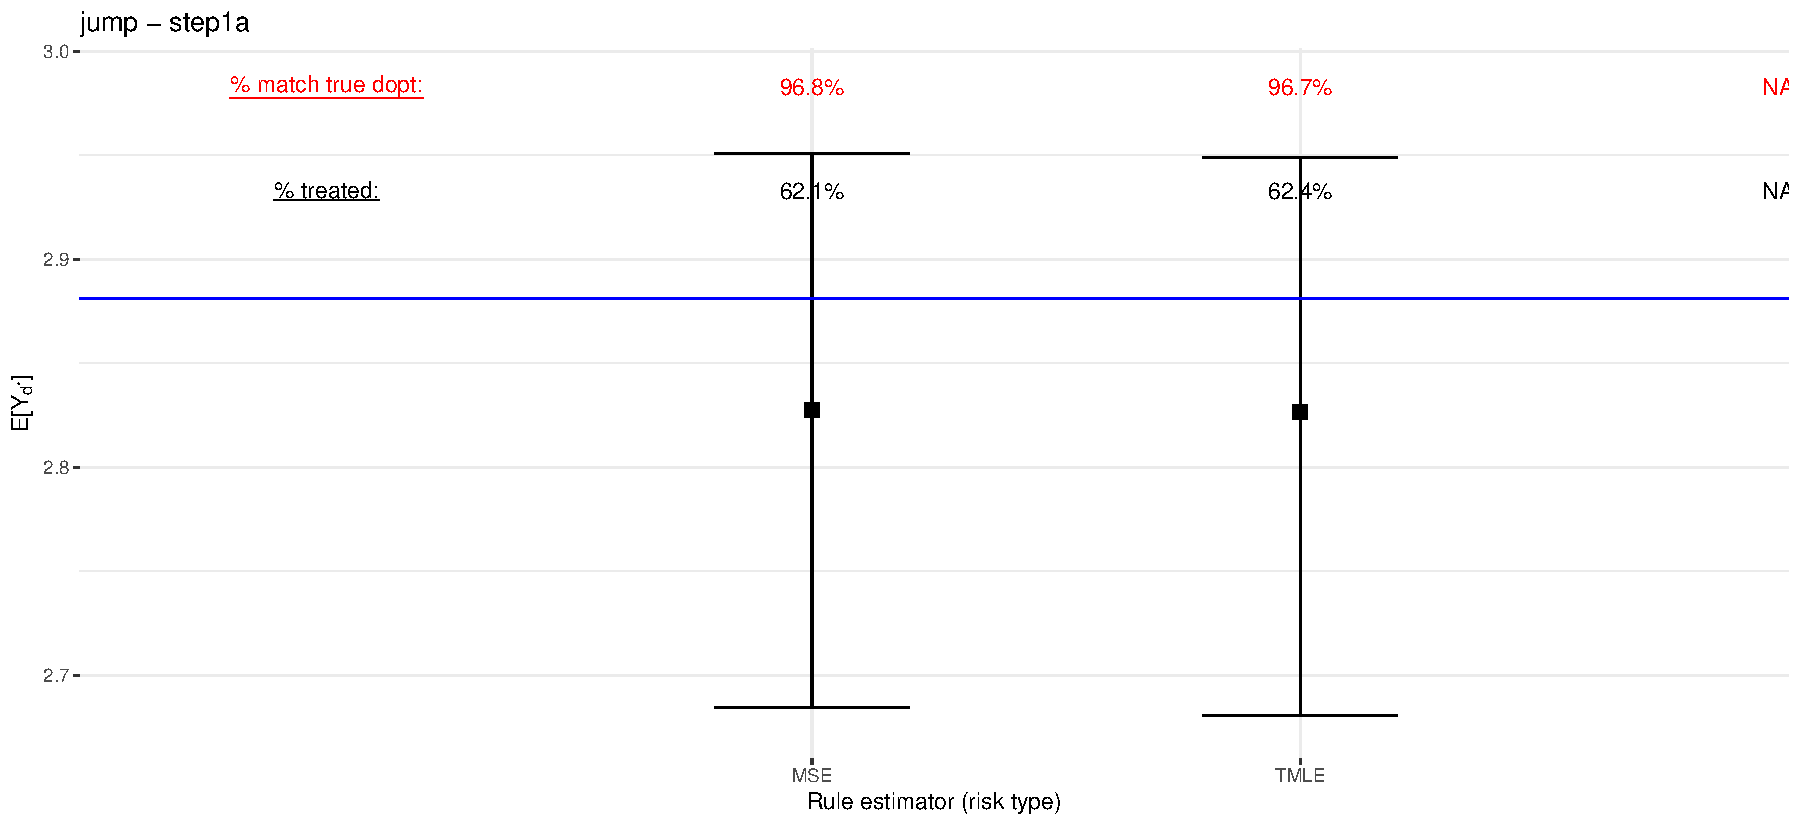
\includegraphics[width=\maxwidth]{figure/ODTR_DGP_jump_step1a-1} 
% latex table generated in R 3.5.1 by xtable 1.8-4 package
% Sat Sep  7 11:01:59 2019
\begin{table}[ht]
\centering
\scalebox{0.8}{
\begin{tabular}{rrr}
  \hline
 & MSE & TMLE \\ 
  \hline
Bias & -0.05378 & -0.05470 \\ 
  Variance & 0.00586 & 0.00466 \\ 
  MSE & 0.00875 & 0.00765 \\ 
  coef.SL.glm & 0.14699 & 0.11458 \\ 
  coef.SL.mean & 0.04465 & 0.13949 \\ 
  coef.SL.glm.interaction & 0.06114 & 0.09331 \\ 
  coef.SL.earth & 0.11612 & 0.12141 \\ 
  coef.SL.nnet & 0.40014 & 0.22561 \\ 
  coef.SL.svm & 0.06508 & 0.09737 \\ 
  coef.SL.rpart & 0.16588 & 0.20823 \\ 
   \hline
\end{tabular}
}
\caption{jump - step1a} 
\end{table}


\subsection{vote-based SL (b)}

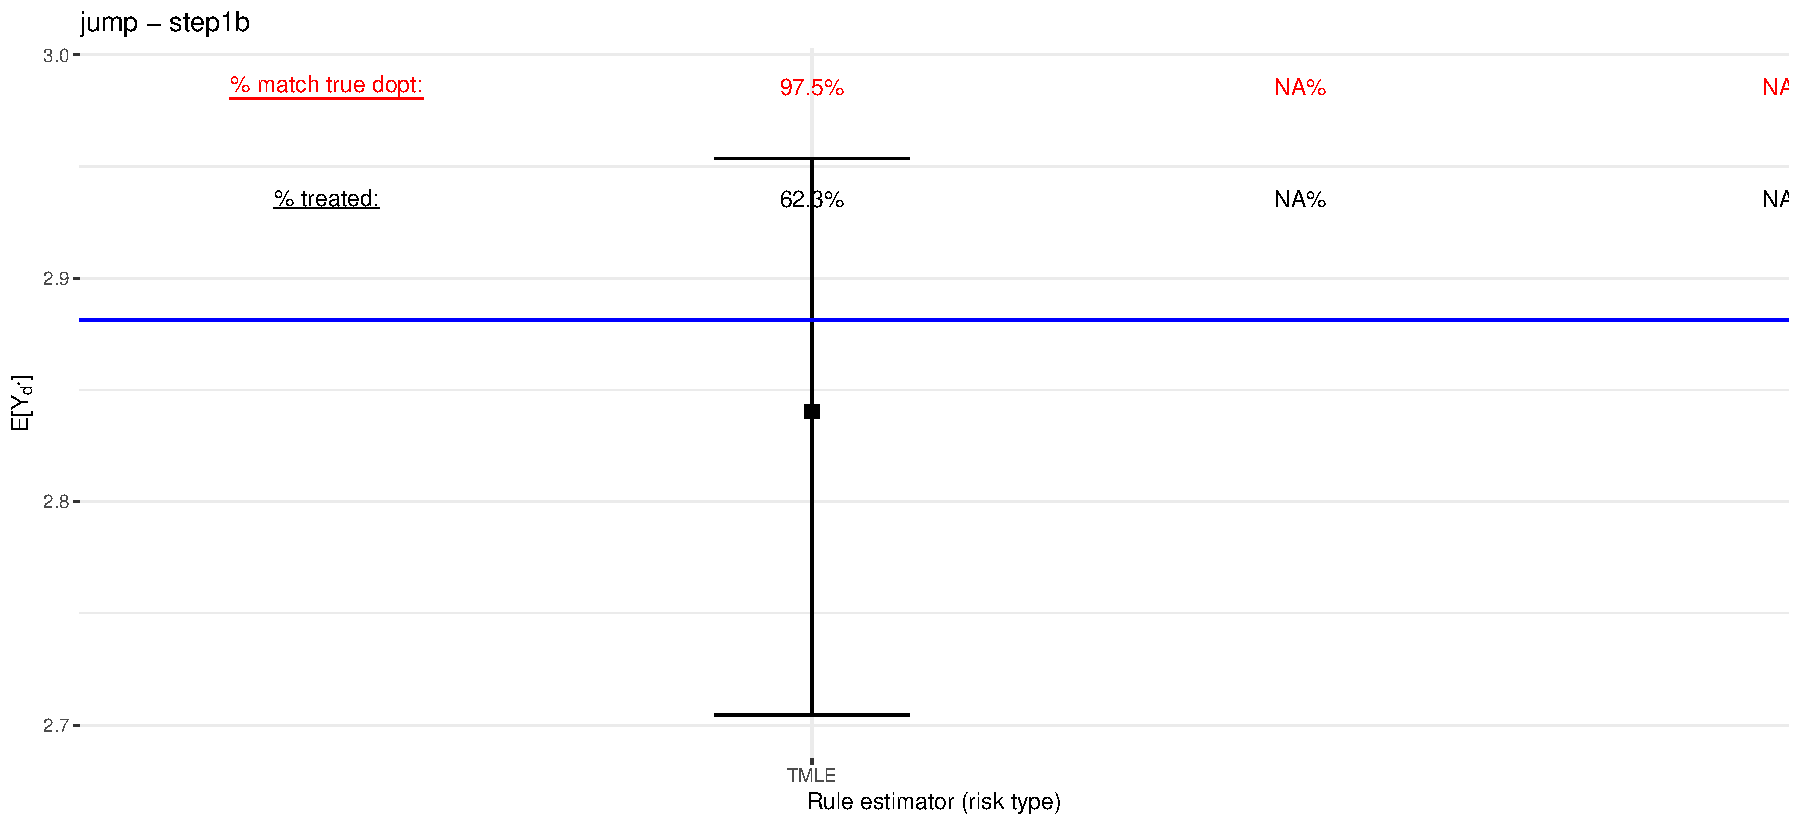
\includegraphics[width=\maxwidth]{figure/ODTR_DGP_jump_step1b-1} 
% latex table generated in R 3.5.1 by xtable 1.8-4 package
% Sat Sep  7 11:02:00 2019
\begin{table}[ht]
\centering
\scalebox{0.7}{
\begin{tabular}{rr}
  \hline
 & TMLE \\ 
  \hline
Bias & -0.04090 \\ 
  Variance & 0.00380 \\ 
  MSE & 0.00547 \\ 
  coef.DonV.DonV.SL.glm\_All & 0.02505 \\ 
  coef.DonV.DonV.SL.mean\_All & 0.04141 \\ 
  coef.DonV.DonV.SL.glm.interaction\_All & 0.02834 \\ 
  coef.DonV.DonV.SL.earth\_All & 0.04695 \\ 
  coef.DonV.DonV.SL.nnet\_All & 0.05050 \\ 
  coef.DonV.DonV.SL.svm\_All & 0.03660 \\ 
  coef.DonV.DonV.SL.rpart\_All & 0.12815 \\ 
  coef.Qlearn.Qlearn.SL.glm\_All & 0.04434 \\ 
  coef.Qlearn.Qlearn.SL.mean\_All & 0.04067 \\ 
  coef.Qlearn.Qlearn.SL.glm.interaction\_All & 0.02534 \\ 
  coef.Qlearn.Qlearn.SL.earth\_All & 0.03875 \\ 
  coef.Qlearn.Qlearn.SL.nnet\_All & 0.04016 \\ 
  coef.Qlearn.Qlearn.SL.svm\_All & 0.03591 \\ 
  coef.Qlearn.Qlearn.SL.rpart\_All & 0.06685 \\ 
  coef.OWL & 0.04362 \\ 
  coef.EARL & 0.02692 \\ 
  coef.optclass & 0.16482 \\ 
  coef.RWL & 0.03084 \\ 
  coef.treatall & 0.04379 \\ 
  coef.treatnone & 0.04099 \\ 
   \hline
\end{tabular}
}
\caption{jump - step1b} 
\end{table}








\section{Step 5}

\begin{itemize}
\item blip (a) and majority vote (b) SuperLearner
\item incorrect glm QAV, incorrect glm QAW
\end{itemize}



\subsection{Blip-based SL (a)}

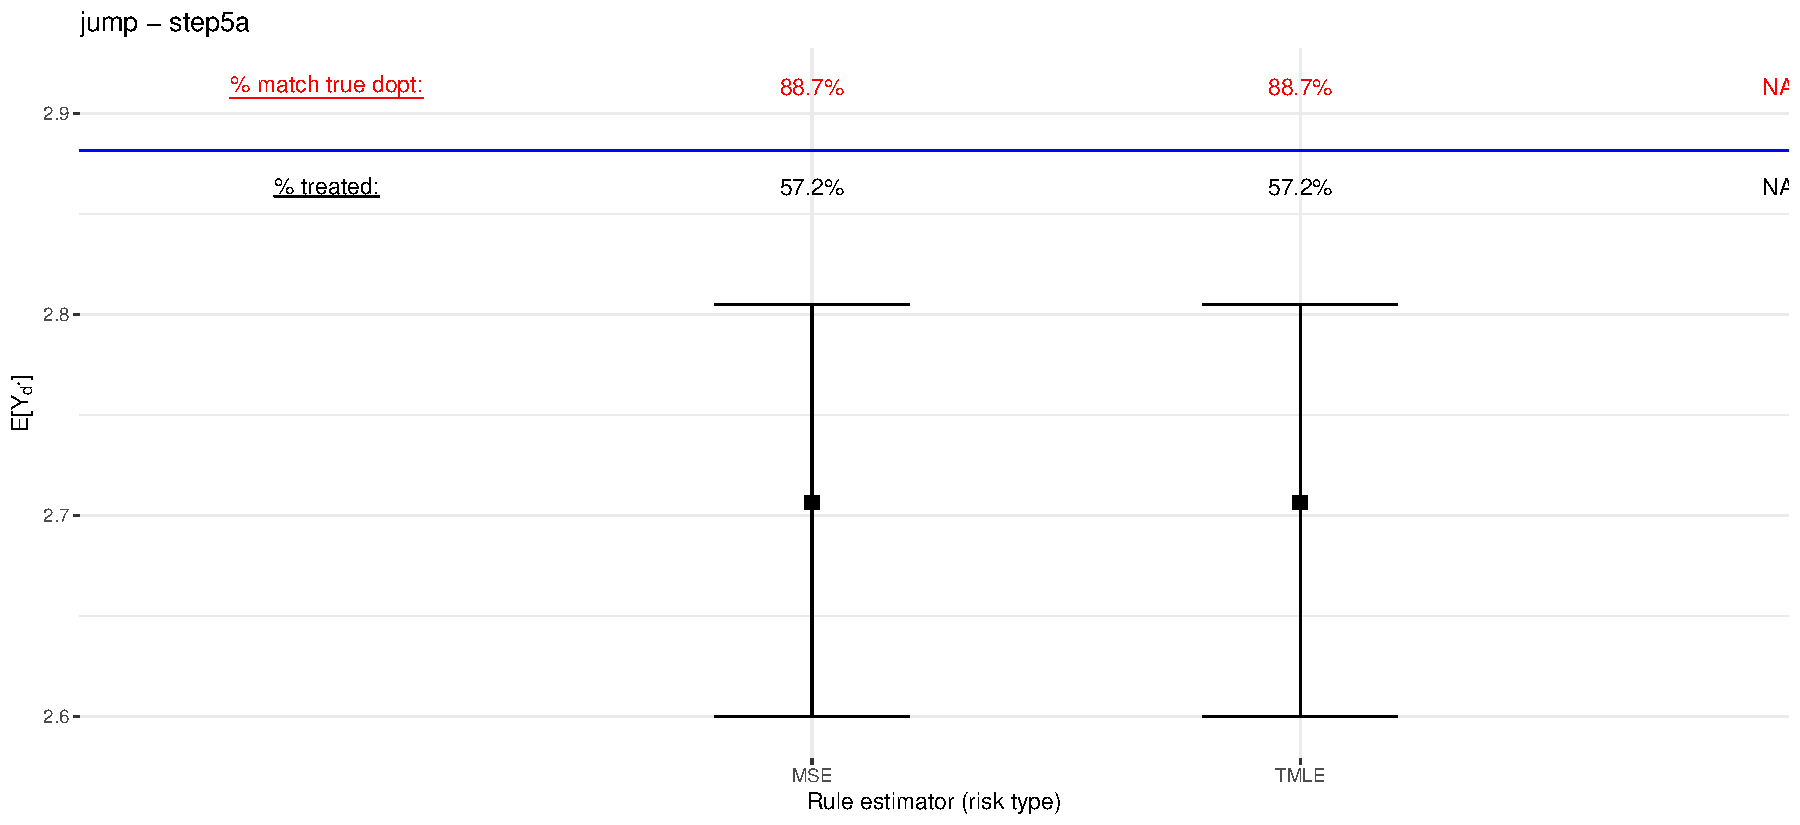
\includegraphics[width=\maxwidth]{figure/ODTR_DGP_jump_step5a-1} 
% latex table generated in R 3.5.1 by xtable 1.8-4 package
% Sat Sep  7 11:02:00 2019
\begin{table}[ht]
\centering
\scalebox{0.7}{
\begin{tabular}{rrr}
  \hline
 & MSE & TMLE \\ 
  \hline
Bias & -0.17497 & -0.17497 \\ 
  Variance & 0.00275 & 0.00275 \\ 
  MSE & 0.03336 & 0.03336 \\ 
  estimates..1.....grep.colnames.estimates..1.....pattern....coef... & 1.00000 & 1.00000 \\ 
   \hline
\end{tabular}
}
\caption{jump - step5a} 
\end{table}


\subsection{vote-based SL (b)}

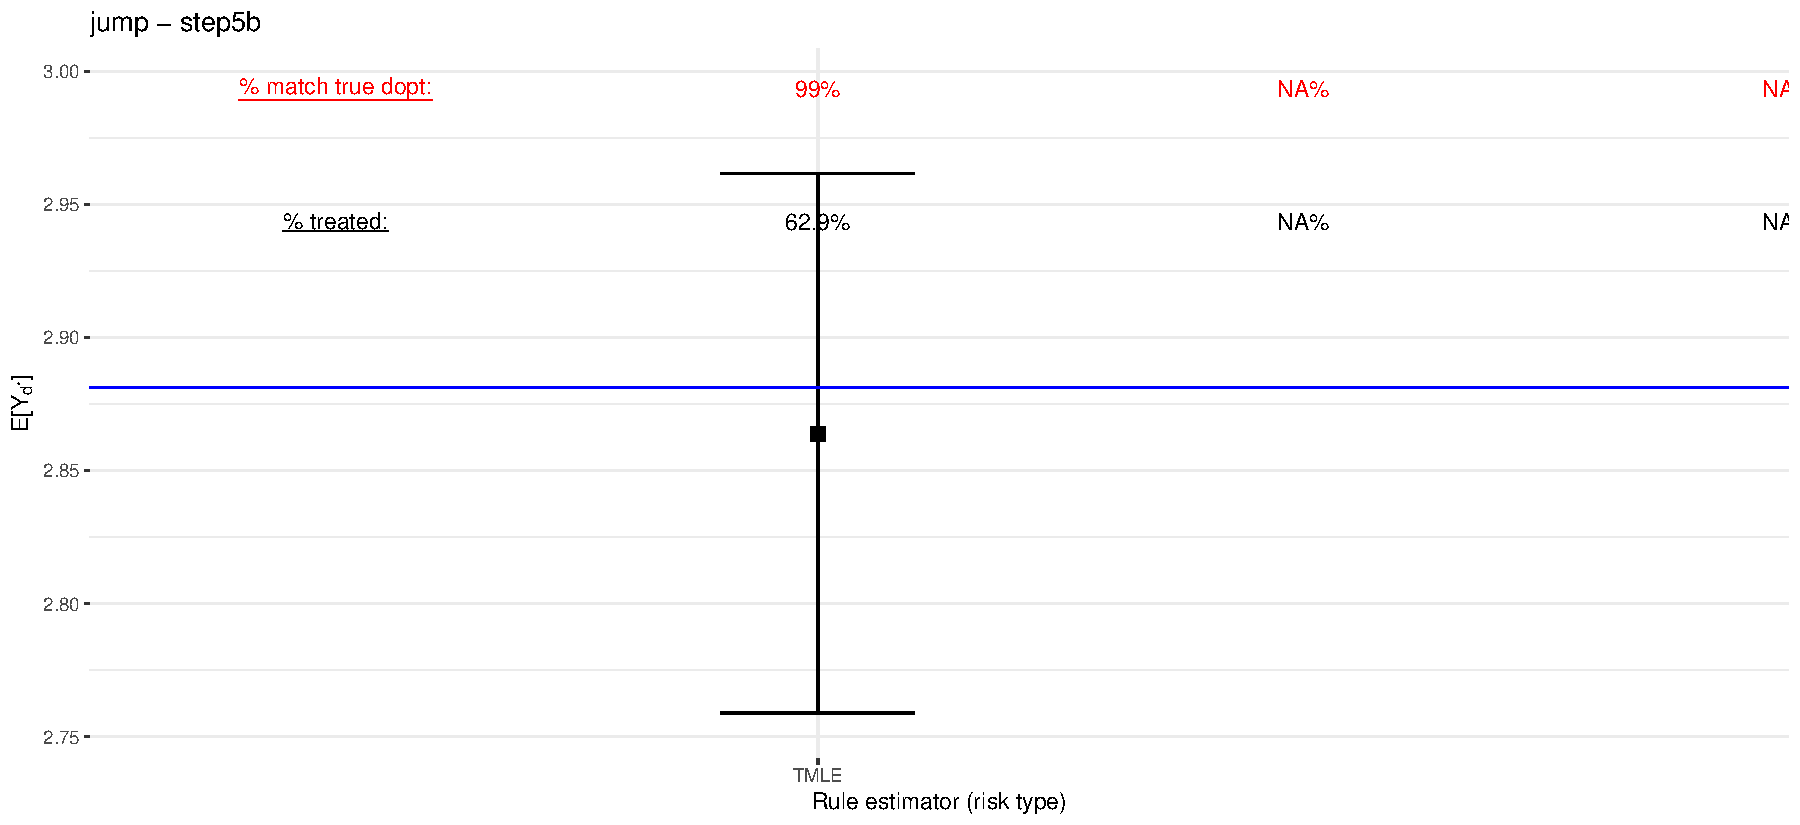
\includegraphics[width=\maxwidth]{figure/ODTR_DGP_jump_step5b-1} 
% latex table generated in R 3.5.1 by xtable 1.8-4 package
% Sat Sep  7 11:02:00 2019
\begin{table}[ht]
\centering
\scalebox{0.7}{
\begin{tabular}{rr}
  \hline
 & TMLE \\ 
  \hline
Bias & -0.01759 \\ 
  Variance & 0.00281 \\ 
  MSE & 0.00312 \\ 
  coef.DonV.SL.glm\_All & 0.02398 \\ 
  coef.Qlearn.SL.QAW.incorrect\_All & 0.02613 \\ 
  coef.OWL & 0.04719 \\ 
  coef.EARL & 0.03596 \\ 
  coef.optclass & 0.74239 \\ 
  coef.RWL & 0.04182 \\ 
  coef.treatall & 0.05089 \\ 
  coef.treatnone & 0.03163 \\ 
   \hline
\end{tabular}
}
\caption{jump - step5a} 
\end{table}


\end{document}
